\subsection{Cross-dataset transfer to HOT3D}
\label{sec:cross}

\paragraph{HOT3D-IF}
HOT3D~\cite{banerjee2025hot3d} shares 21 objects with identical canonical meshes, the UmeTrack hand skeleton~\cite{han2022umetrack} and the Quest~3 headset with SHOW3D, which makes it the only public dataset on which the joint-anchored field can be generated with the same code path and no joint-convention mapping. Its Quest~3 clips differ in three respects that we resolve: they are raw fisheye streams at 30\,fps, annotated with UmeTrack wrist poses and joint angles rather than landmarks, and each frame contains several objects. We rectify both streams through the Fisheye624 model (a Kannala-Brandt polynomial~\cite{kannala2006generic} with tangential and thin-prism terms) to SHOW3D's virtual pinhole camera ($1024\times1280$, focal length 454\,px, principal point centred, rotated so that hands appear below and the left hand on the left), recover landmarks by UmeTrack forward kinematics from the per-clip hand shape (our implementation reproduces SHOW3D's stored landmarks to within $10^{-4}$\,mm), map objects by name to SHOW3D aliases (posed SHOW3D meshes project into HOT3D's own annotated boxes within one pixel, confirming that the canonical frames coincide), and define the target object of a hand as the nearest shared object within 150\,mm. Fields, camera-frame joints, visibility and observability then follow the SHOW3D derivation exactly. Participants are split into HOT3D-train (P0002, P0003, P0010, P0013) and HOT3D-eval (P0017, P0018, P0021); training clips are the only ones with ground truth, so evaluation uses a disjoint set of training-split participants. We extract 63 clips (nine per participant, 150 source frames each, which the 10\,fps stride reduces to 50) and a further 120 clips of the training participants, giving 9,150 frames of which 6,855 are labelled; at the 5\,fps stride of the token models this yields 2,889 training frames and 538 evaluation frames (17,598 joint targets). The HOT3D field is lighter-tailed than SHOW3D's (median 35.0\,mm, mean 50.8\,mm in the initial 63-clip build) and hands are further from the camera (median joint depth 378 against 308\,mm), so HOT3D-eval is an easier set in absolute terms and only differences between models trained identically are informative.

\begin{table*}[t]
\centering\small
\caption{Cross-dataset results (mean ADE in mm and accuracies). Each block trains on the data in the first column and is evaluated on SHOW3D fold-A validation and on HOT3D-eval. The SHOW3D block re-uses the fold-A checkpoints of \cref{tab:main}; the HOT3D-train block trains on 2,889 frames and stopped early after six epochs; the joint block trains on the union. The zero-vector predictor scores 82.6\,mm on SHOW3D fold A.}
\label{tab:transfer}
\begin{tabular}{@{}llrrrrr@{}}
\toprule
 & & \multicolumn{2}{c}{SHOW3D fold A} & \multicolumn{3}{c}{HOT3D-IF eval} \\
\cmidrule(lr){3-4}\cmidrule(lr){5-7}
Training data & Model & ADE & acc@50 & ADE & acc@10 & acc@50 \\
\midrule
SHOW3D (37,645 frames) & Direct, single view (B2) & 49.58 & 0.742 & 38.98 & 0.202 & 0.787 \\
 & Direct, stereo (B3) & 46.15 & 0.756 & 40.18 & 0.201 & 0.777 \\
 & FIF, geometric head only & 55.11 & 0.689 & 50.32 & 0.072 & 0.665 \\
 & FIF (full) & 44.43 & 0.768 & 43.91 & 0.183 & 0.763 \\
\midrule
HOT3D-train (2,889 frames) & Direct, stereo & 78.13 & 0.671 & 42.63 & 0.087 & 0.750 \\
 & FIF (full) & 79.59 & 0.661 & 43.32 & 0.082 & 0.748 \\
\midrule
SHOW3D + HOT3D-train (40,534) & Direct, stereo & 46.20 & 0.760 & 34.54 & 0.221 & 0.818 \\
 & FIF (full) & 46.16 & 0.766 & 36.71 & 0.171 & 0.806 \\
\bottomrule
\end{tabular}

\end{table*}

\begin{figure}[t]
\centering
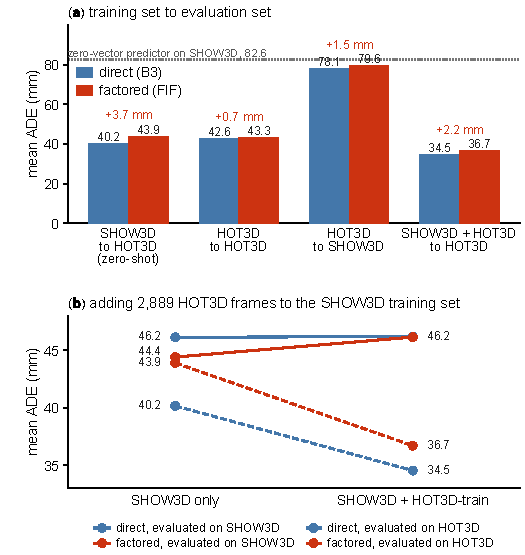
\includegraphics[width=\columnwidth]{../figures/fig9_transfer.pdf}
\caption{Cross-dataset transfer between SHOW3D and HOT3D-IF. (a) Direct against factored model in the four cross-dataset settings; the annotation is the difference (positive: factored worse). (b) The effect of adding the 2,889 HOT3D-train frames to the SHOW3D training set, evaluated on both datasets: the direct model is unchanged on SHOW3D and improves on HOT3D; the factored model loses its SHOW3D margin and improves less on HOT3D.}
\label{fig:transfer}
\end{figure}

\paragraph{Zero-shot transfer}
\Cref{tab:transfer} and \cref{fig:transfer}a report the fold-A checkpoints applied to HOT3D-eval without any adaptation. Every model does better on HOT3D than on SHOW3D, as expected from its lighter tail, but by very different amounts: the single-view direct regressor improves from 49.6 to 39.0\,mm, the stereo direct regressor from 46.2 to 40.2\,mm, and the factored model from 44.4 to only 43.9\,mm. The in-domain ranking inverts exactly: the best SHOW3D model is the worst on HOT3D, and the simplest model transfers best. The factored model is 3.7\,mm behind the matched direct regressor.

\paragraph{Training on HOT3D and joint training}
Training on HOT3D-train alone gives 42.6\,mm (direct) and 43.3\,mm (factored) on HOT3D-eval, both \emph{worse} than the SHOW3D-trained models applied zero-shot: 37,645 frames of another dataset beat 2,889 frames of the same one. Applied in the reverse direction these models reach 78.1 and 79.6\,mm on SHOW3D, barely below the 82.6\,mm of the zero-vector predictor, so the small HOT3D set does not support a transferable model at all, and the transfer is asymmetric for reasons of scale rather than of domain. Adding HOT3D-train to the SHOW3D training set is the best-powered comparison. It leaves the direct model unchanged on SHOW3D (46.15 to 46.20\,mm) and improves it on HOT3D by 5.6\,mm (40.2 to 34.5\,mm). It costs the factored model 1.7\,mm on SHOW3D (44.43 to 46.16\,mm), exactly its in-domain margin, and improves it on HOT3D by 7.2\,mm to 36.7\,mm, still 2.2\,mm behind the direct model (\cref{fig:transfer}b). After joint training the two models are tied on SHOW3D and the factored one is behind on HOT3D; the stratified gains of \cref{fig:strata} vanish as well (0.9 and 0.6\,mm \emph{against} the factored model in the near and middle strata, 1.5\,mm against it on occluded joints). The third clause of the falsification criterion therefore fails in all four settings, and the advantage of geometric supervision is confined to training on a single dataset.

\paragraph{Where the transfer fails}
The head-wise numbers locate the loss. On HOT3D the factored model's direct head alone scores 42.1\,mm against 40.2\,mm for the standalone direct regressor, so 1.9 of the 3.7\,mm are a property of the representation: the geometric supervision that helped on SHOW3D made the shared decoder more specific to SHOW3D. The remaining 1.8\,mm come from the fusion, whose weight on a geometric head that now scores 63.5\,mm cannot fall below the floor set by the saturated scale. Replacing the predicted object pose by the ground truth does not help the geometric head on HOT3D (63.9 against 63.5\,mm), whereas it helped by 8.7\,mm in domain: out of domain the predicted \emph{joints} are the bottleneck. After joint training this reverses again (38.4\,mm with the true object pose against 53.2), so the joint branch adapts to the new hands once it sees them while the object-pose branch remains the weak link. The mechanism is consistent with the ablations: the factored model's advantage rests on the object-pose branch being useful, and that branch is the least transferable component. That models fit the dataset they are trained on is an old observation~\cite{torralba2011unbiased}; what the present result adds is that a formulation designed to inject dataset-independent geometry can \emph{increase} that dependence when its geometric branch is trained on one distribution of object poses and meshes.

Two caveats apply. HOT3D-eval has 538 frames, so differences below about two millimetres should not be over-read, although the direction is the same in all four settings; and the HOT3D-only models early-stopped after six epochs on a noisy validation set and may be under-trained, which affects the absolute level of the HOT3D-train block but not the joint-training comparison.
